\section{Research Papers}
\label{sec:research-papers}

\subsection{Debugging of RxJS-Based Applications}
\label{sec:paper-1}

This paper was published with the proceedings of the 7th ACM SIGPLAN International Workshop
on Reactive and Event-Based Languages and Systems (REBLS '20), 16th November 2020.

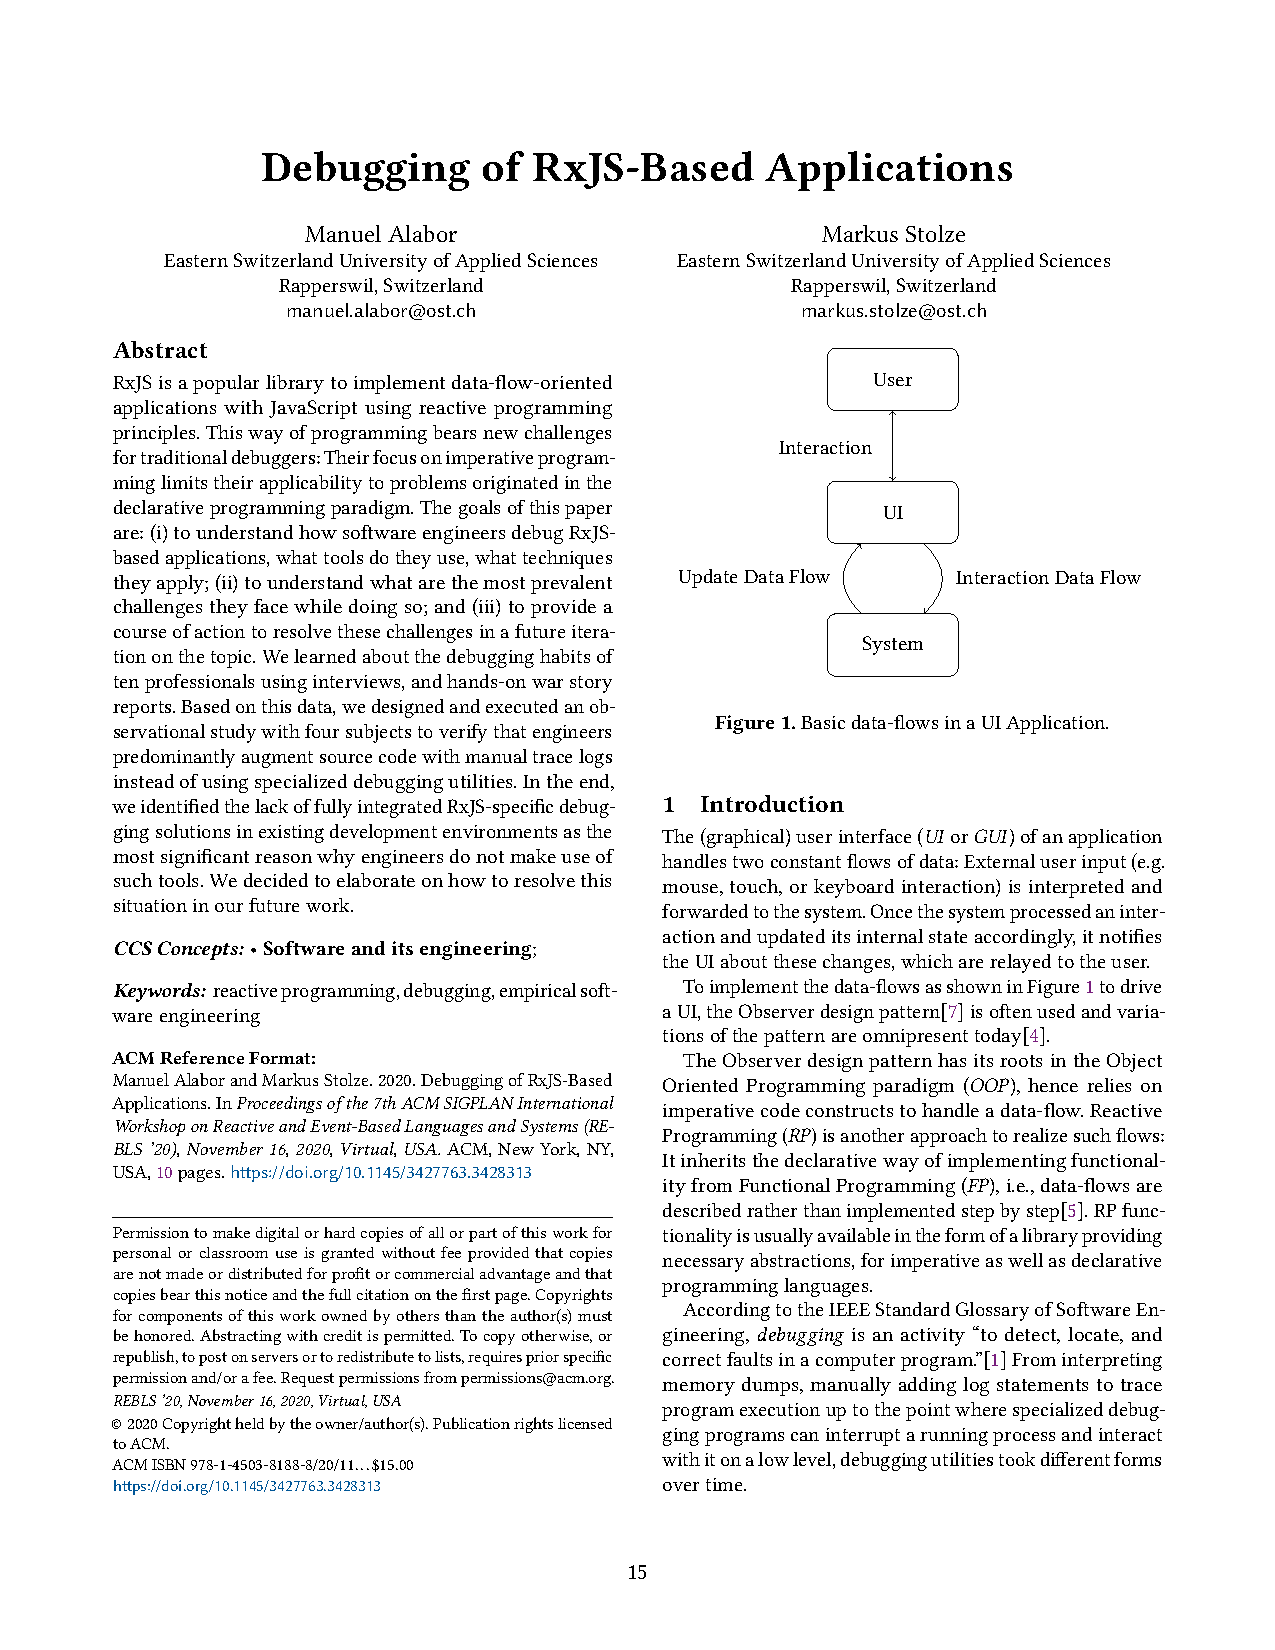
\includepdf[pages=-]{content/pdfs/3427763.3428313.pdf}



\subsection{Debugging Support for Reactive Programming}
\label{sec:paper-2}

The review version of this paper (Appendix \ref{sec:paper-2-paper}) and its supplementary material
(Appendix \ref{sec:paper-2-supplementary}) were submitted to the Technical Papers track at the 31st ACM SIGSOFT
International Symposium on Software Testing and Analysis 2022 (ISSTA '22).

\subsubsection{Paper}
\label{sec:paper-2-paper}
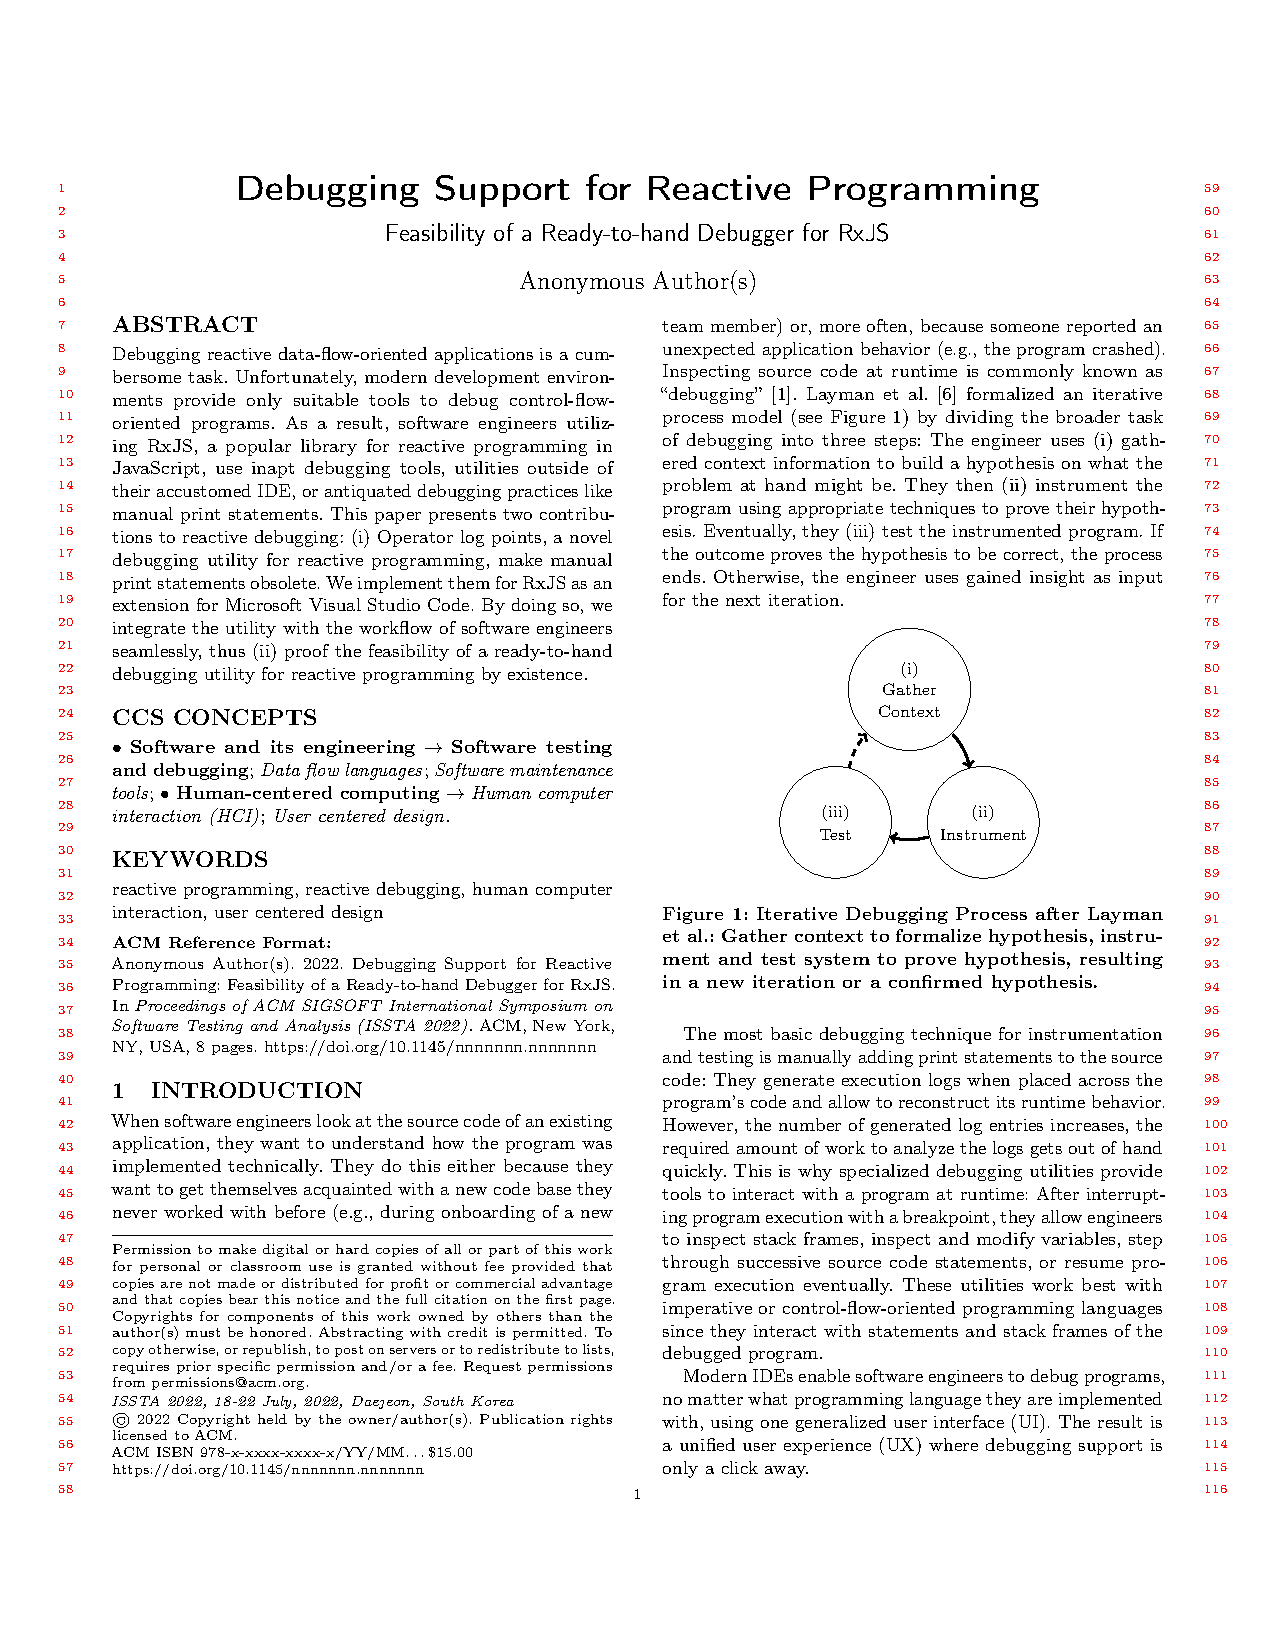
\includepdf[pages=-]{content/pdfs/issta/paper.pdf}

\subsubsection{Supplementary Material}
\label{sec:paper-2-supplementary}
\includepdf[pages=1-12]{content/pdfs/issta/supplementary-material.pdf}
\includepdf[pages=13-14,landscape=true]{content/pdfs/issta/supplementary-material.pdf}
\includepdf[pages=15-]{content/pdfs/issta/supplementary-material.pdf}


\section{Comparative User Journey}
\label{sec:user-journey}

The Comparative User Journey is publicly accessible on alabor.me and GitHub as well:

\begin{itemize}
  \item \url{https://alabor.me/research/user-journey-debugging-of-rxjs-based-applications/}
  \item \url{https://github.com/swissmanu/alabor.me/tree/master/research/user-journey-debugging-of-rxjs-based-applications}
\end{itemize}

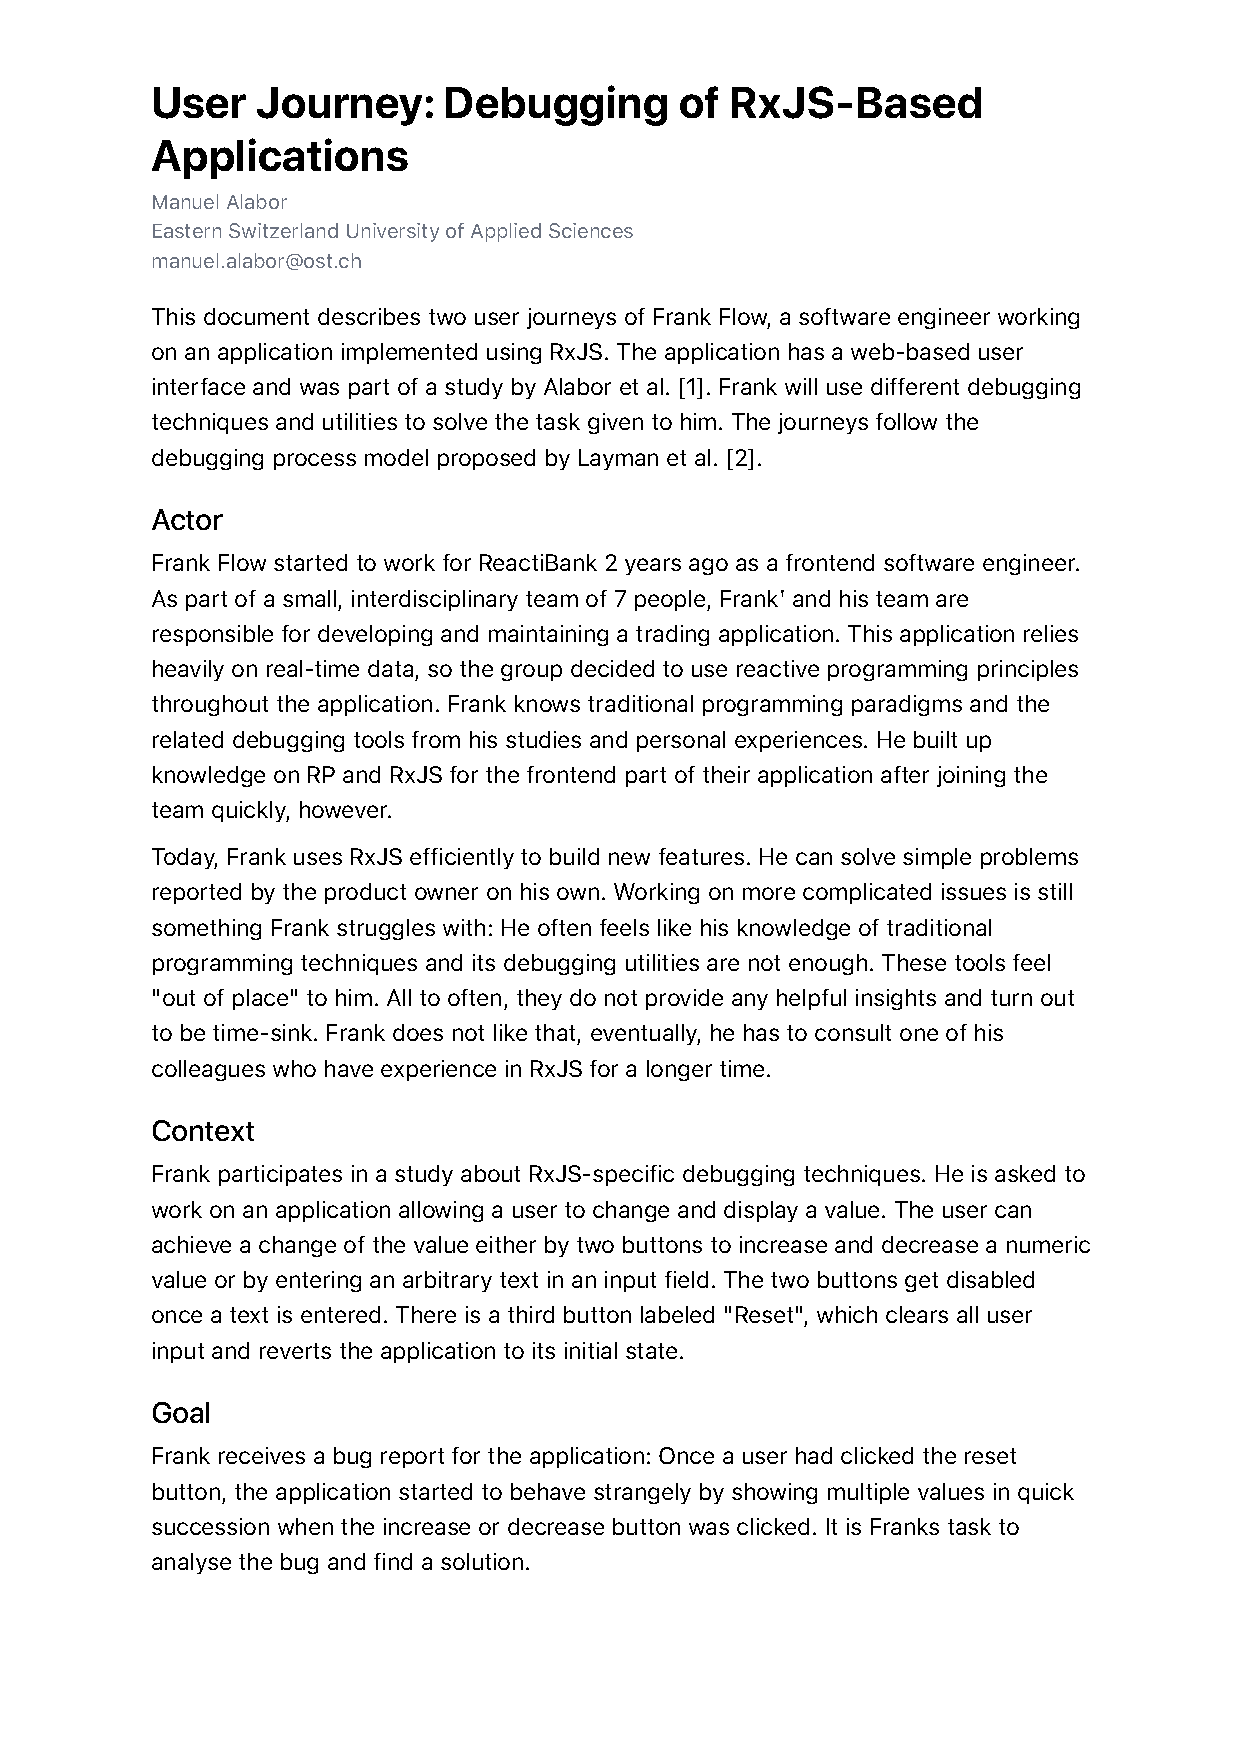
\includepdf[pages=-]{content/pdfs/user-journey.pdf}




\section{RxJS Debugging for vscode}


\subsection{Major Release Milestone Plan}
\label{sec:major-milestone}
The following document was created at the 31th of December, 10:00 CET and is publicly accesible:

\begin{itemize}
  \item \url{https://github.com/swissmanu/rxjs-debugging-for-vscode/milestone/2?closed=1}
\end{itemize}

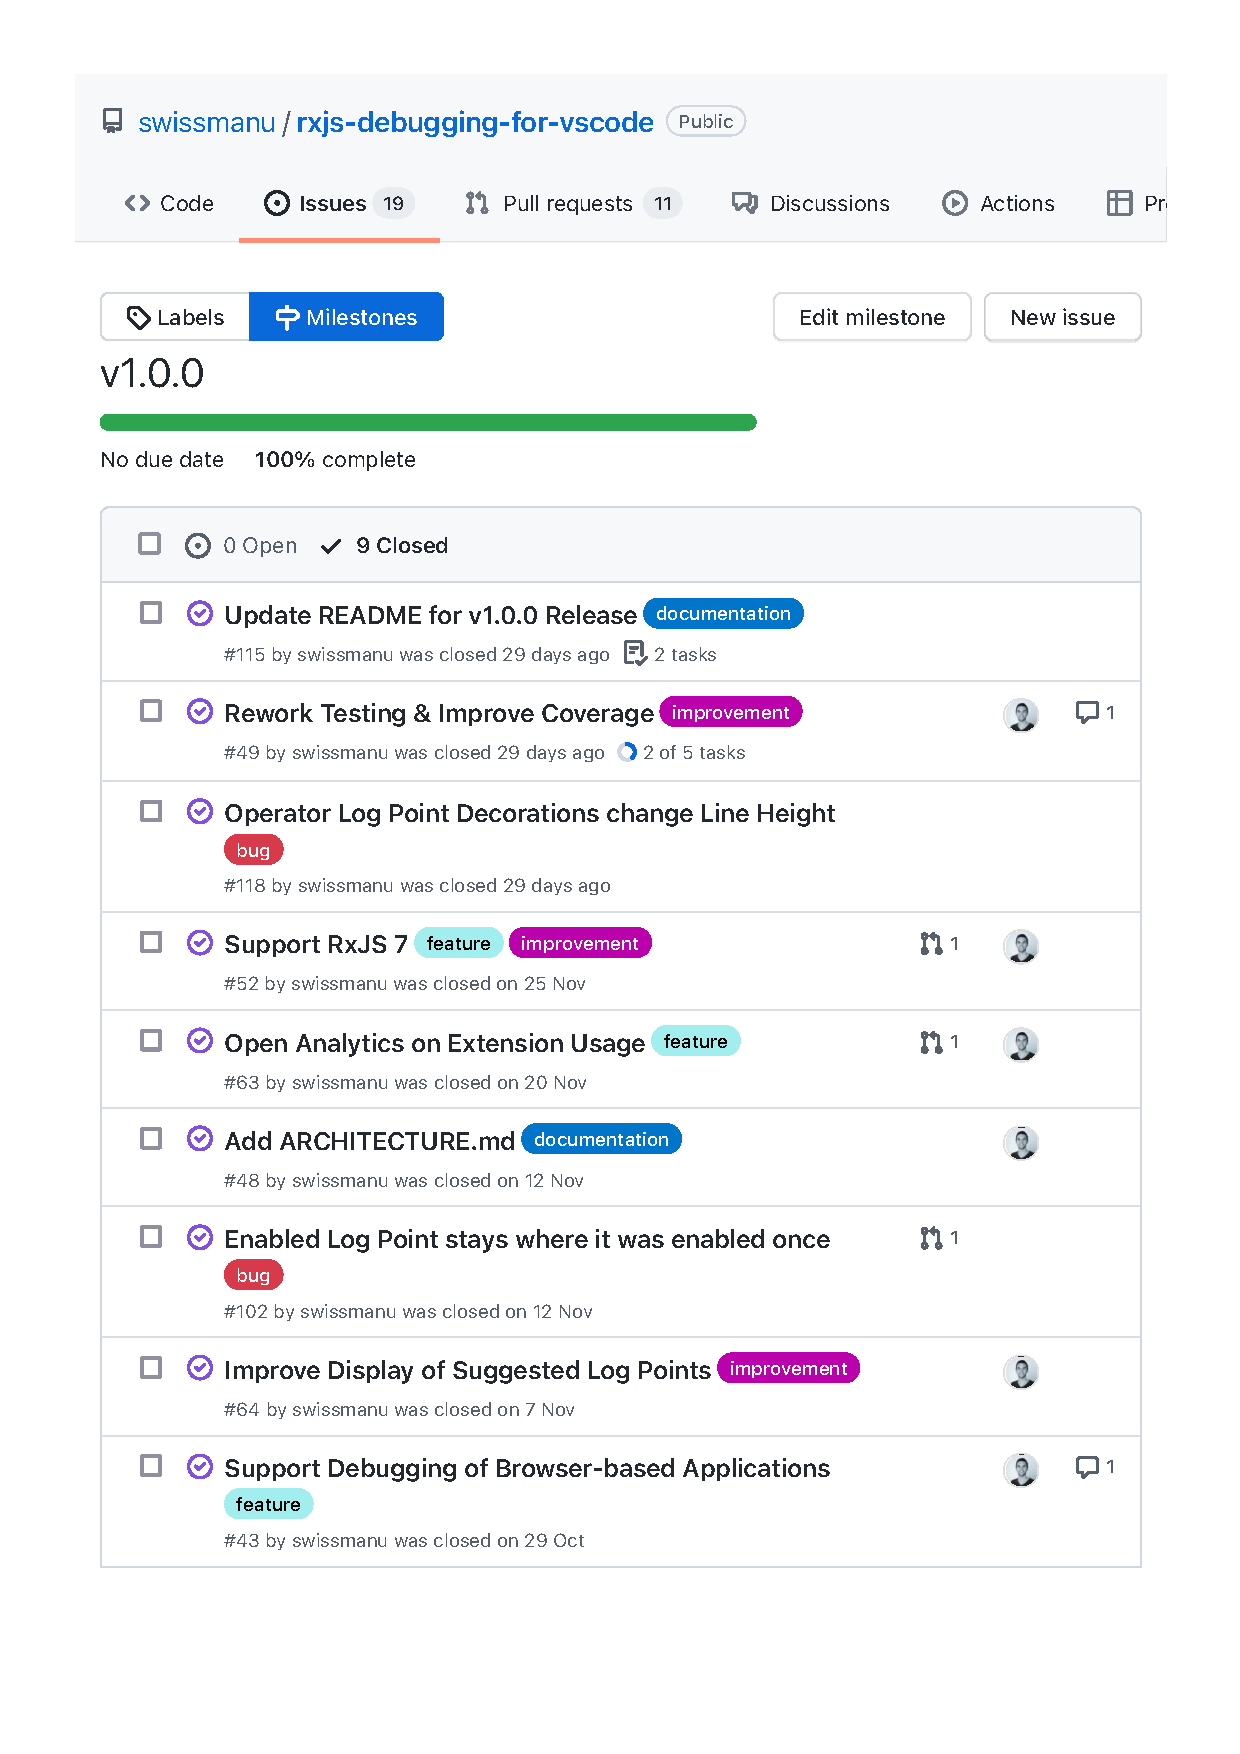
\includepdf[pages=-]{content/pdfs/major-milestone.pdf}




\subsection{Feature Backlog}
\label{sec:feature-backlog}
The following document was created at the 31th of December, 10:00 CET. Its most current version is publicly accesible:

\begin{itemize}
  \item \url{https://github.com/swissmanu/rxjs-debugging-for-vscode/issues?q=is%3Aopen+is%3Aissue+label%3Afeature%2Cimprovement}
\end{itemize}

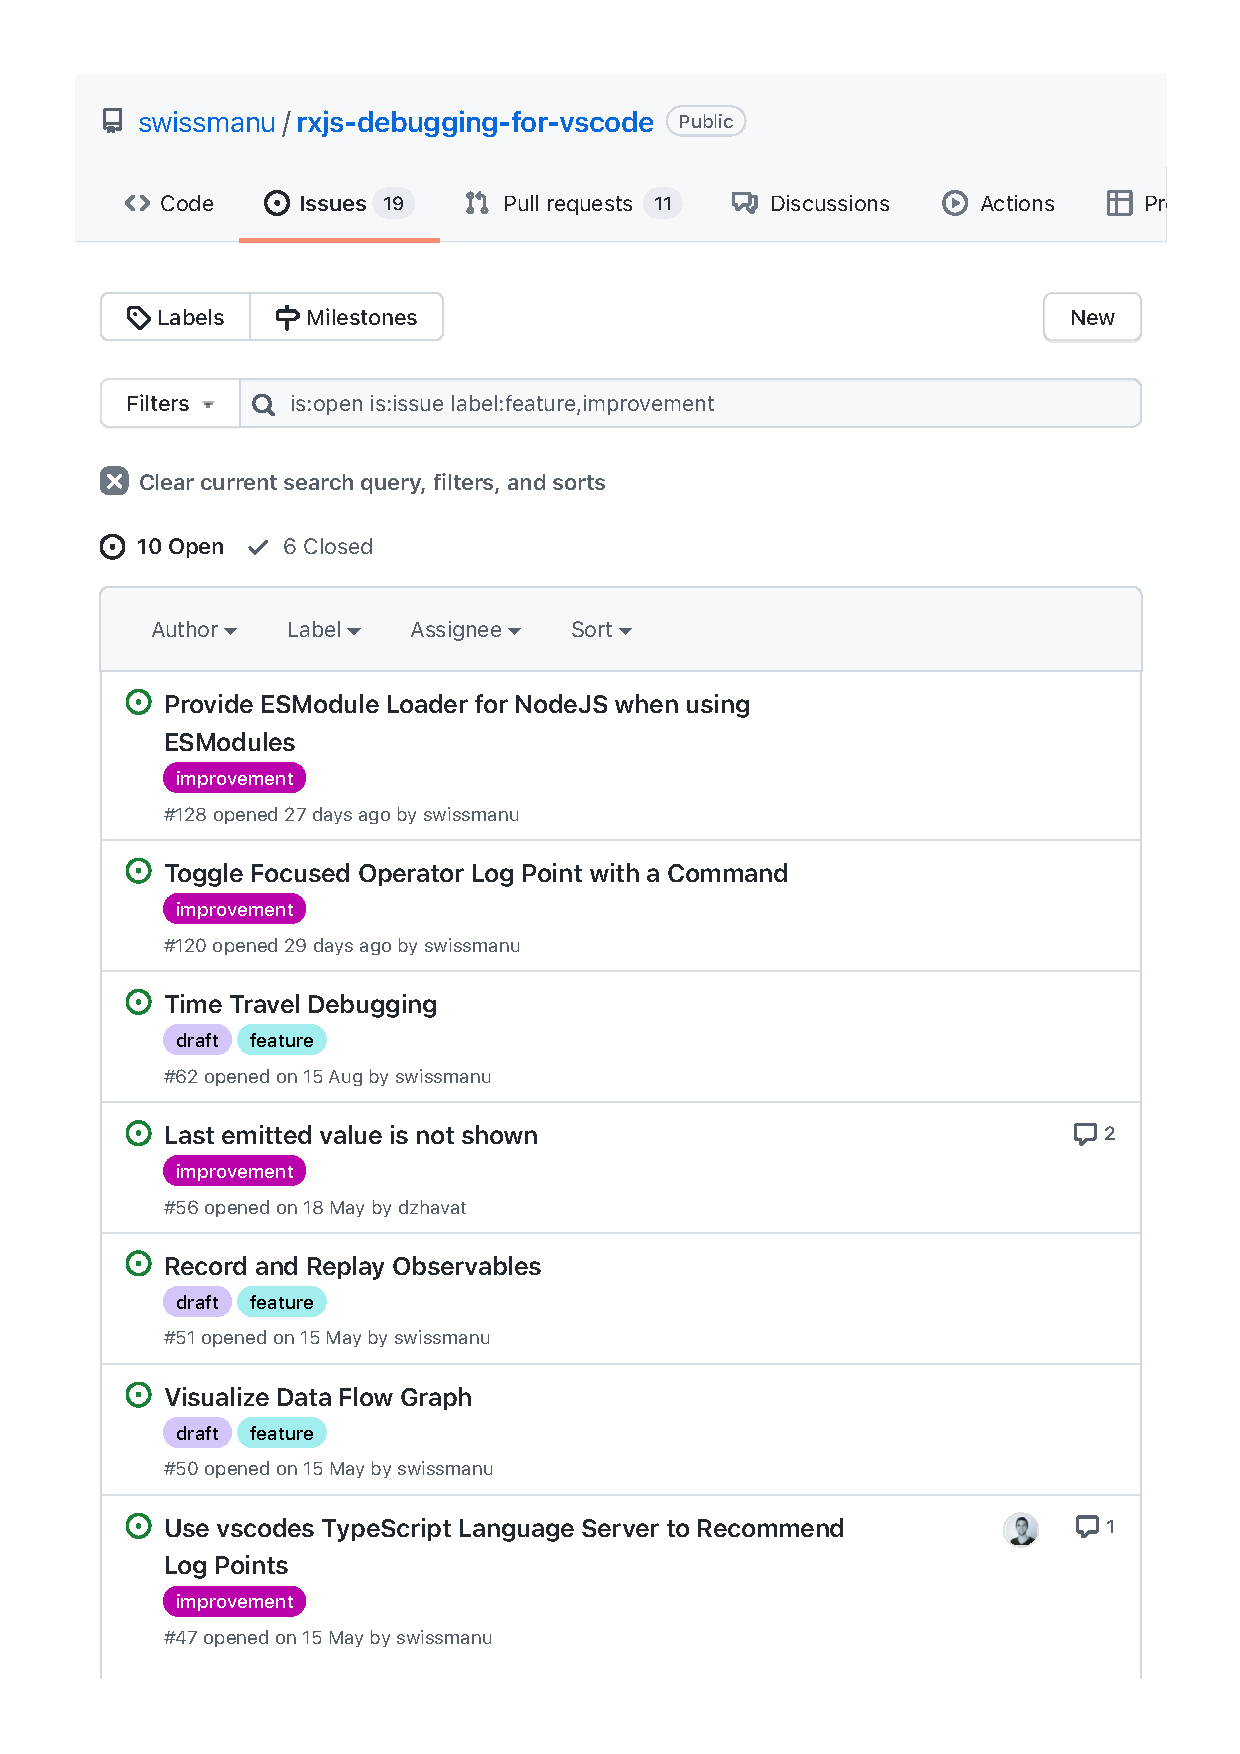
\includepdf[pages=-, landscape=true, nup=2, frame=true]{content/pdfs/feature-backlog.pdf}


\subsection{Release Tweet Stats}
\label{sec:release-tweet-stats}
The following screenshot was taken at the 30th of December, 19:00 CET.

URL of the publicly available tweet:

\begin{itemize}
  \item \url{https://twitter.com/rxjsdebugging/status/1466439953731182599}
\end{itemize}

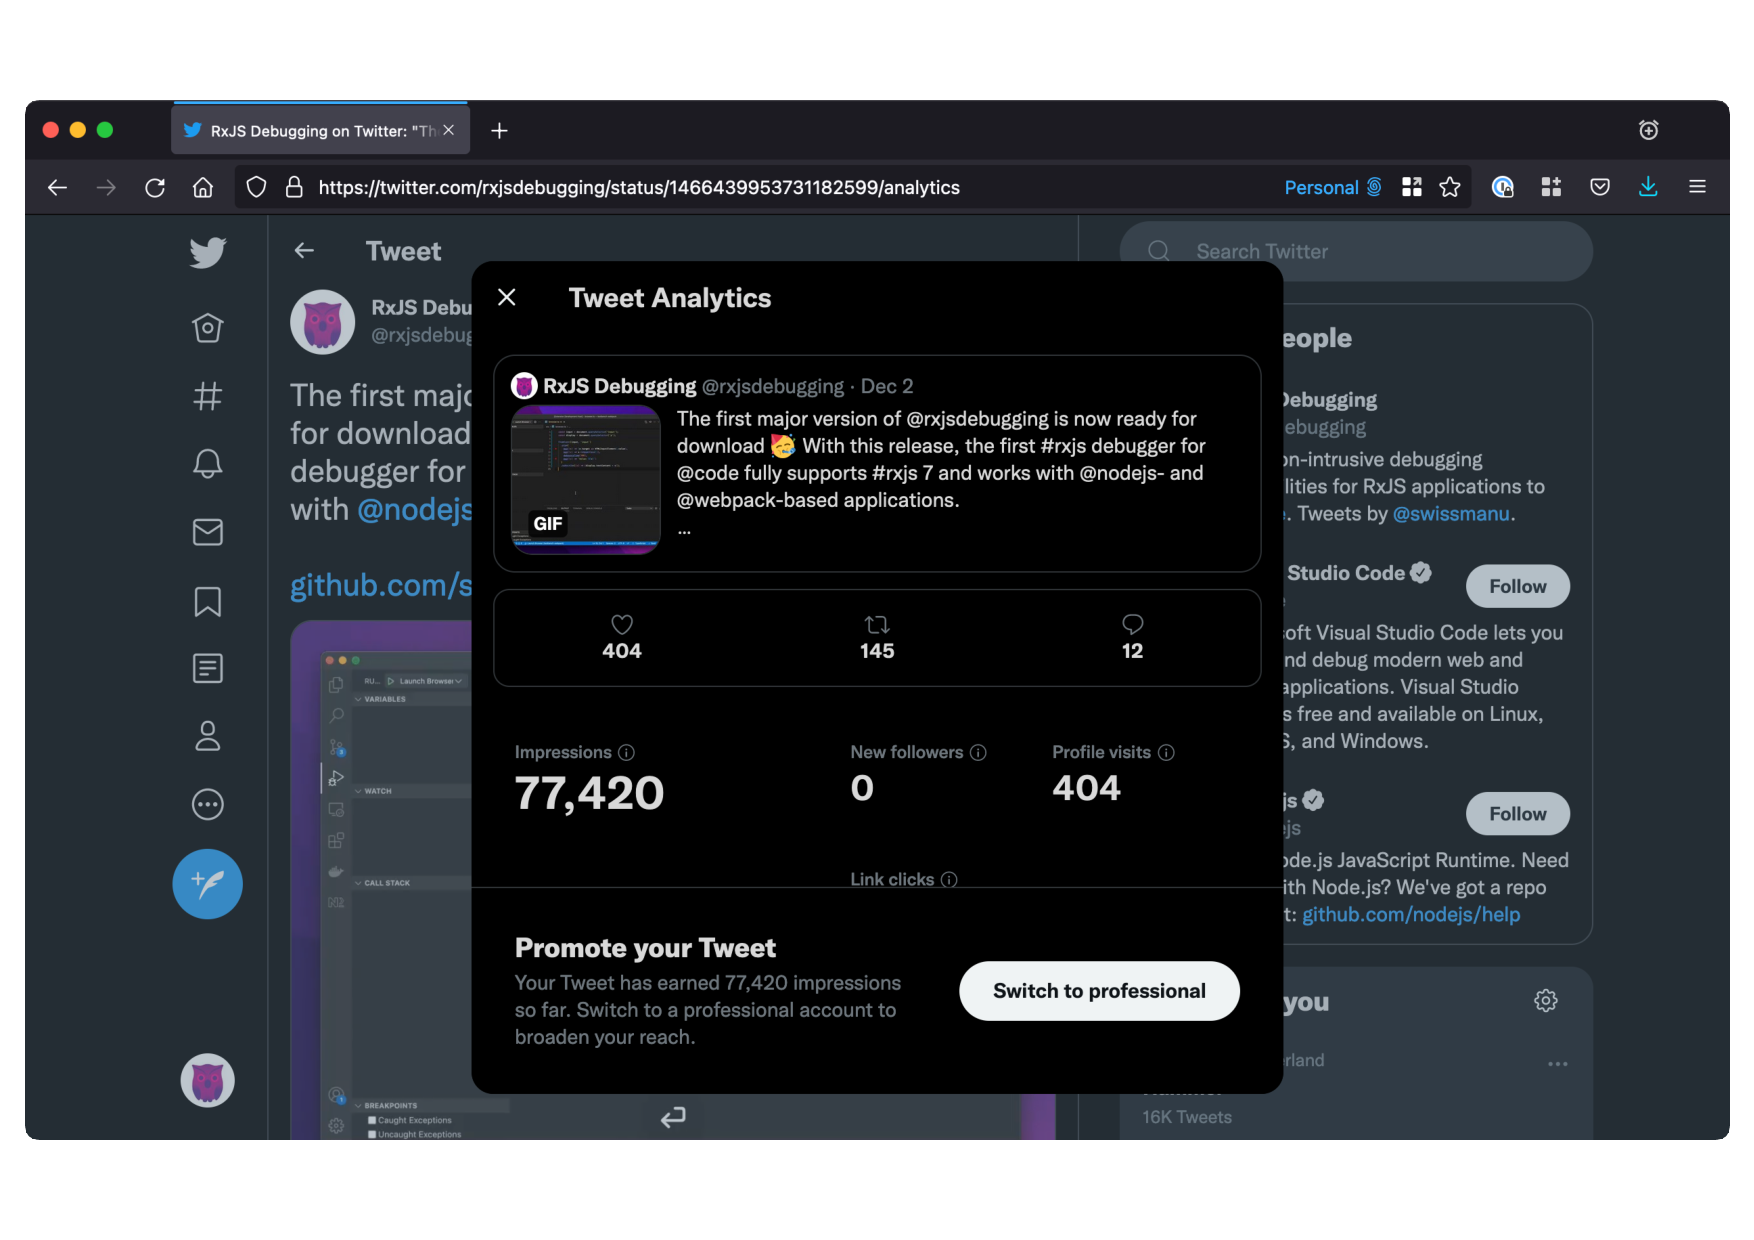
\includepdf[landscape=true,pages=-]{content/pdfs/release-tweet.pdf}


\subsection{Visual Studio Marketplace}
\label{sec:marketplace}
The following screenshots were taken at the 30th of December, 19:00 CET.

URL of the publicly available Marketplace page:

\begin{itemize}
  \item \url{https://marketplace.visualstudio.com/items?itemName=manuelalabor.rxjs-debugging-for-vs-code}
\end{itemize}

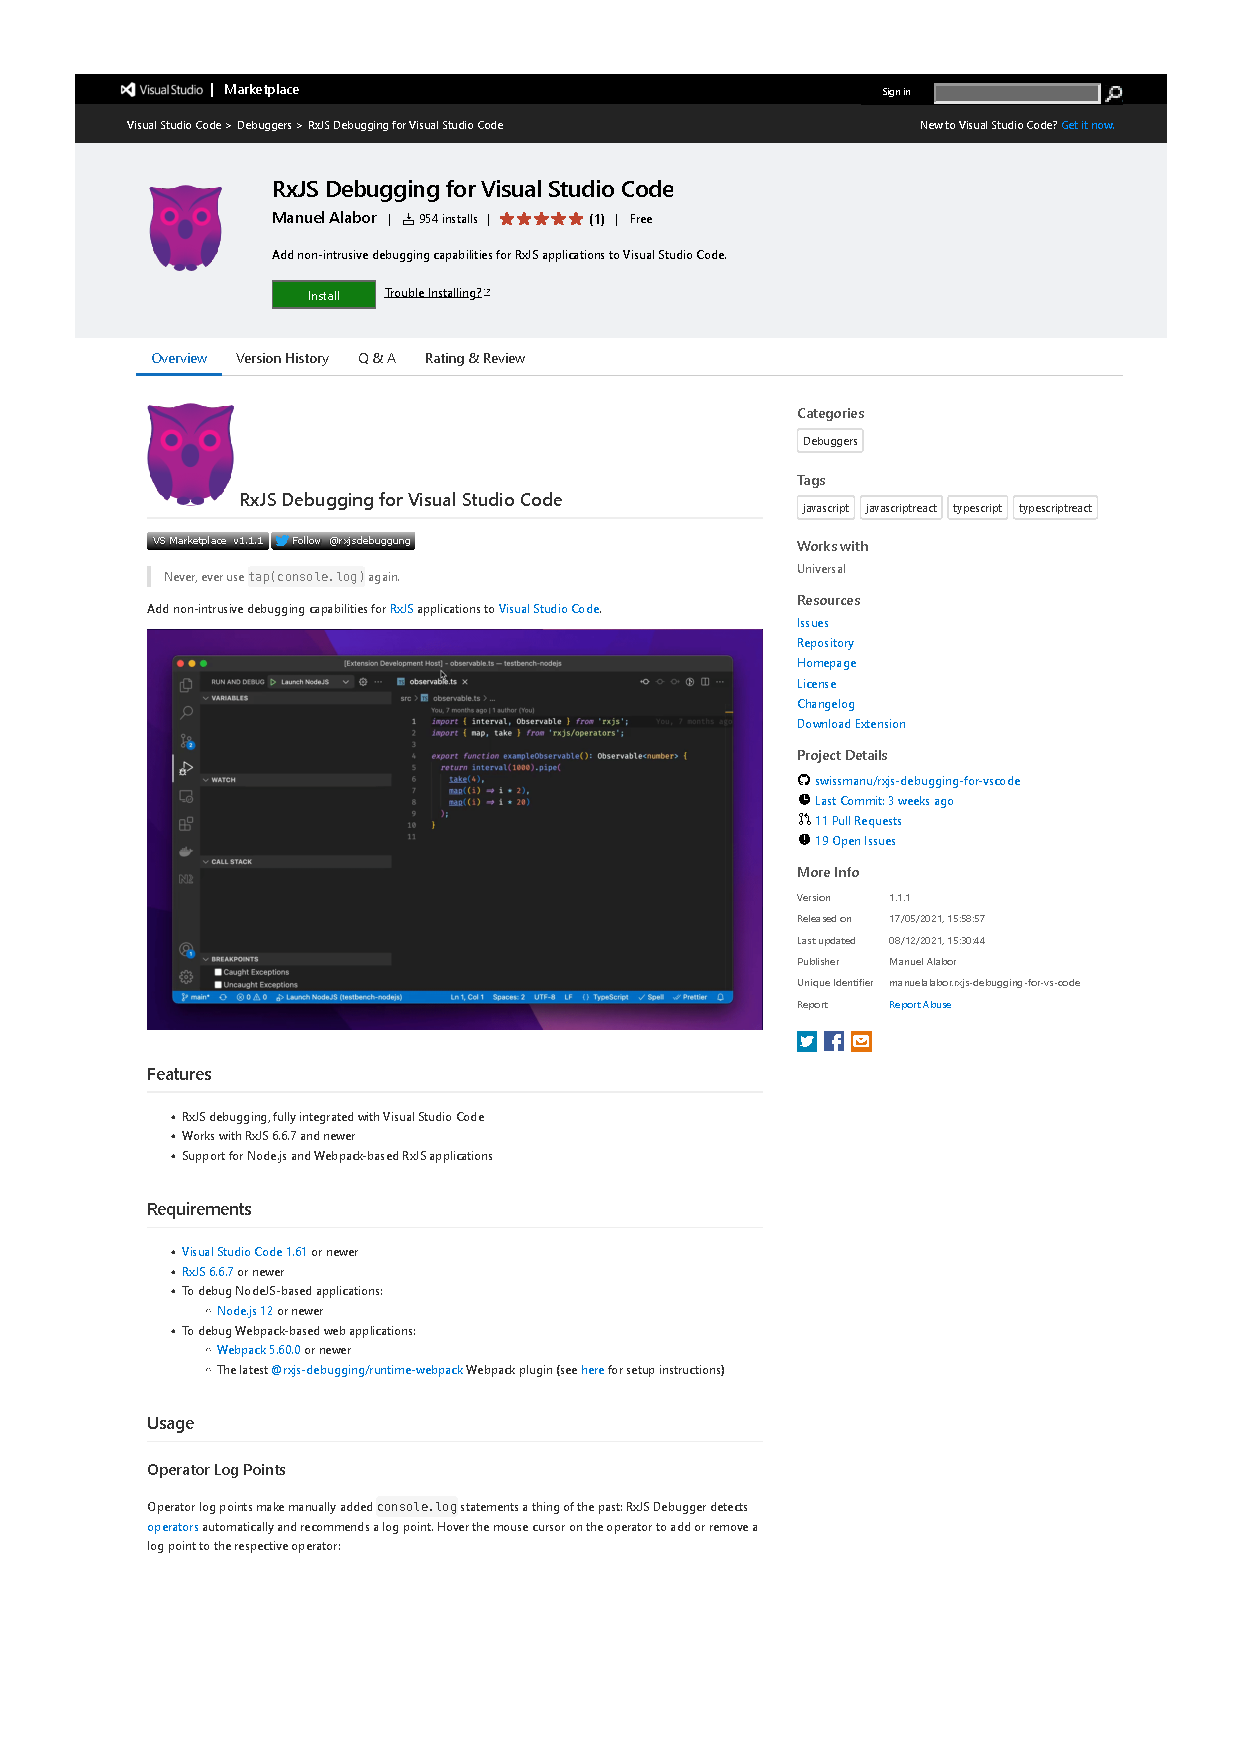
\includepdf[pages=-, landscape=true, nup=2, frame=true]{content/pdfs/marketplace.pdf}



\subsection{ANALYTICS.md}
\label{sec:analytics}
The following document is a snapshot of the ANALYTICS.md file from the Git repository of RxJS Debugging for vscode:

\begin{itemize}
  \item \url{https://github.com/swissmanu/rxjs-debugging-for-vscode/blob/1bb1c20cbf3633ef45cf0df16aacb3c3ea8a8c8c/ANALYTICS.md}
\end{itemize}

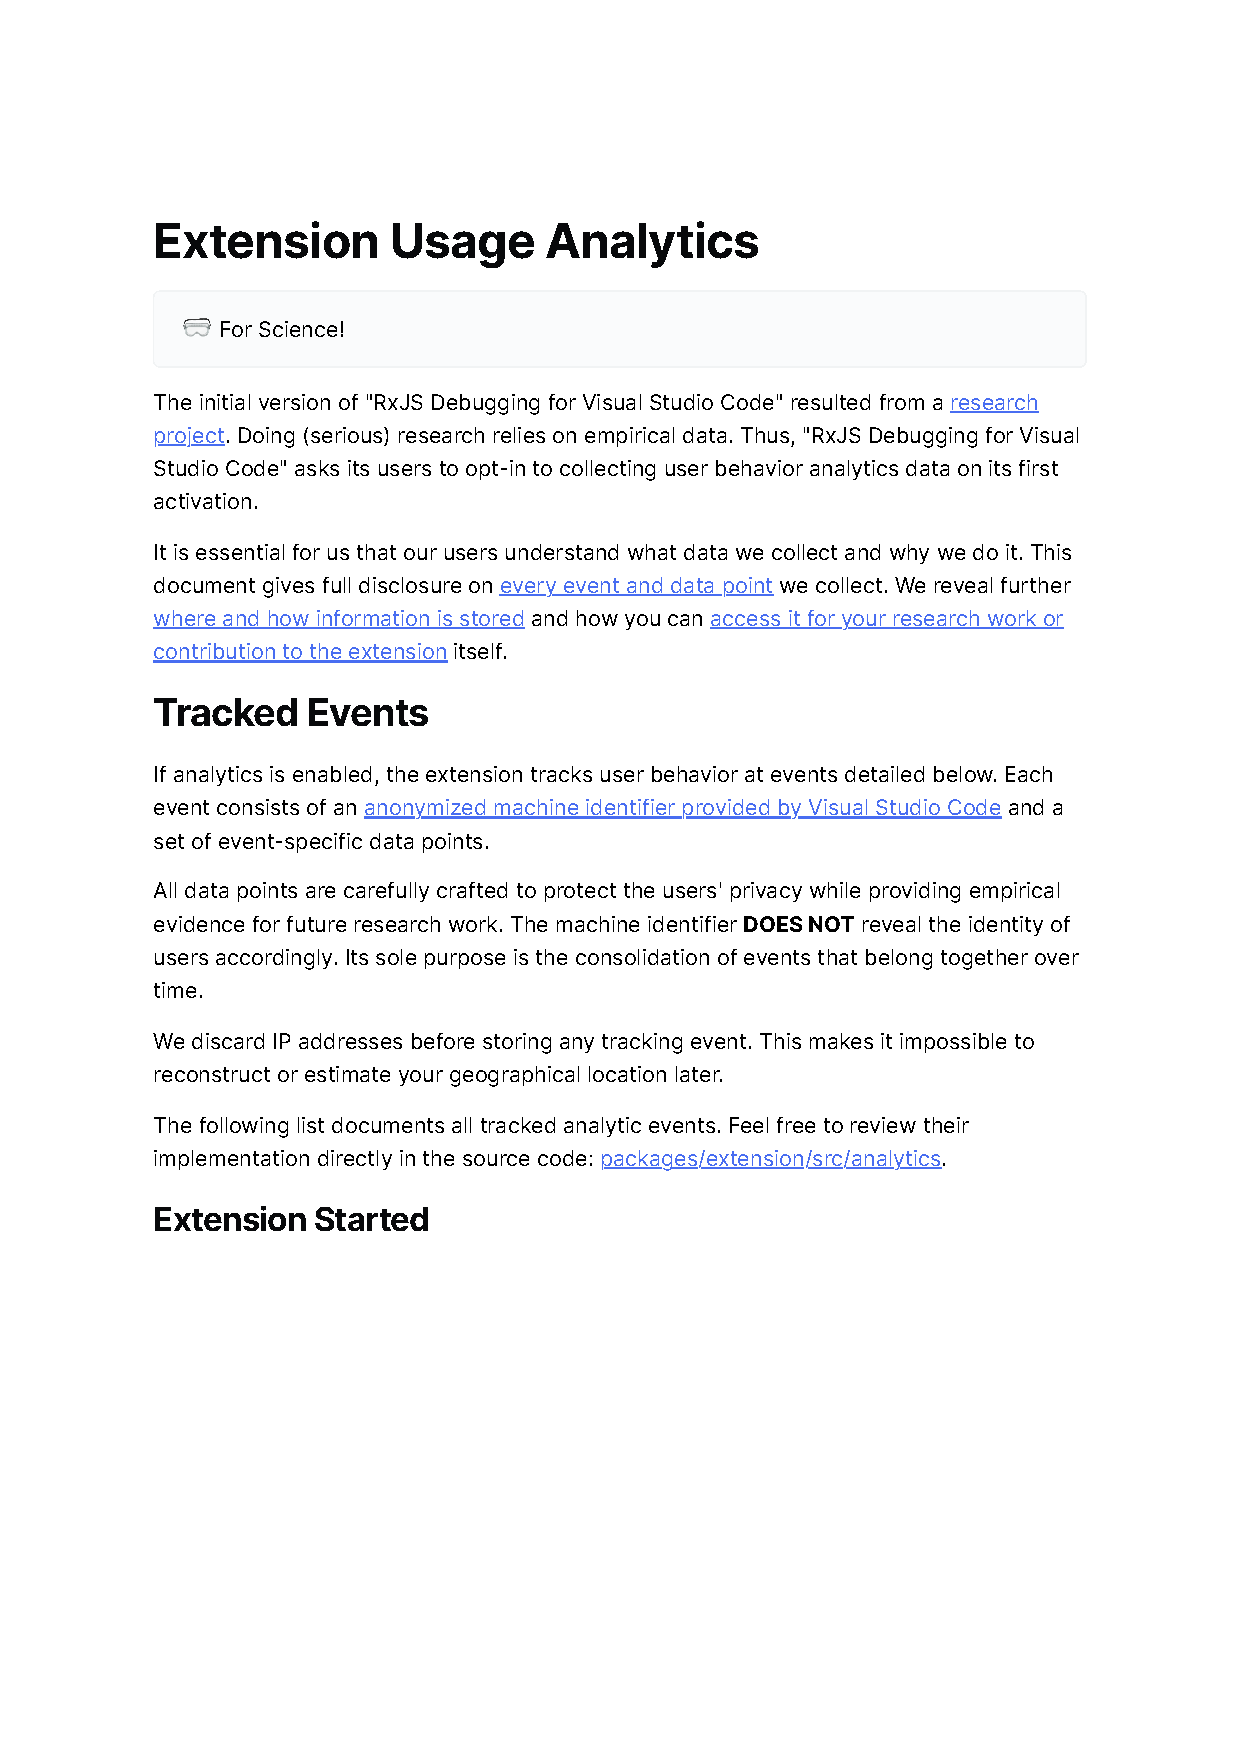
\includepdf[pages=-, landscape=true, nup=2, frame=true]{content/pdfs/analyticsmd.pdf}


\subsection{ARCHITECTURE.md}
\label{sec:architecture}
The following document is a snapshot of the ARCHITECTURE.md file from the Git repository of RxJS Debugging for vscode:

\begin{itemize}
  \item \url{https://github.com/swissmanu/rxjs-debugging-for-vscode/blob/50ca1b93427bd87e6af1a7466b46d1bf669cce6c/ARCHITECTURE.md}
\end{itemize}

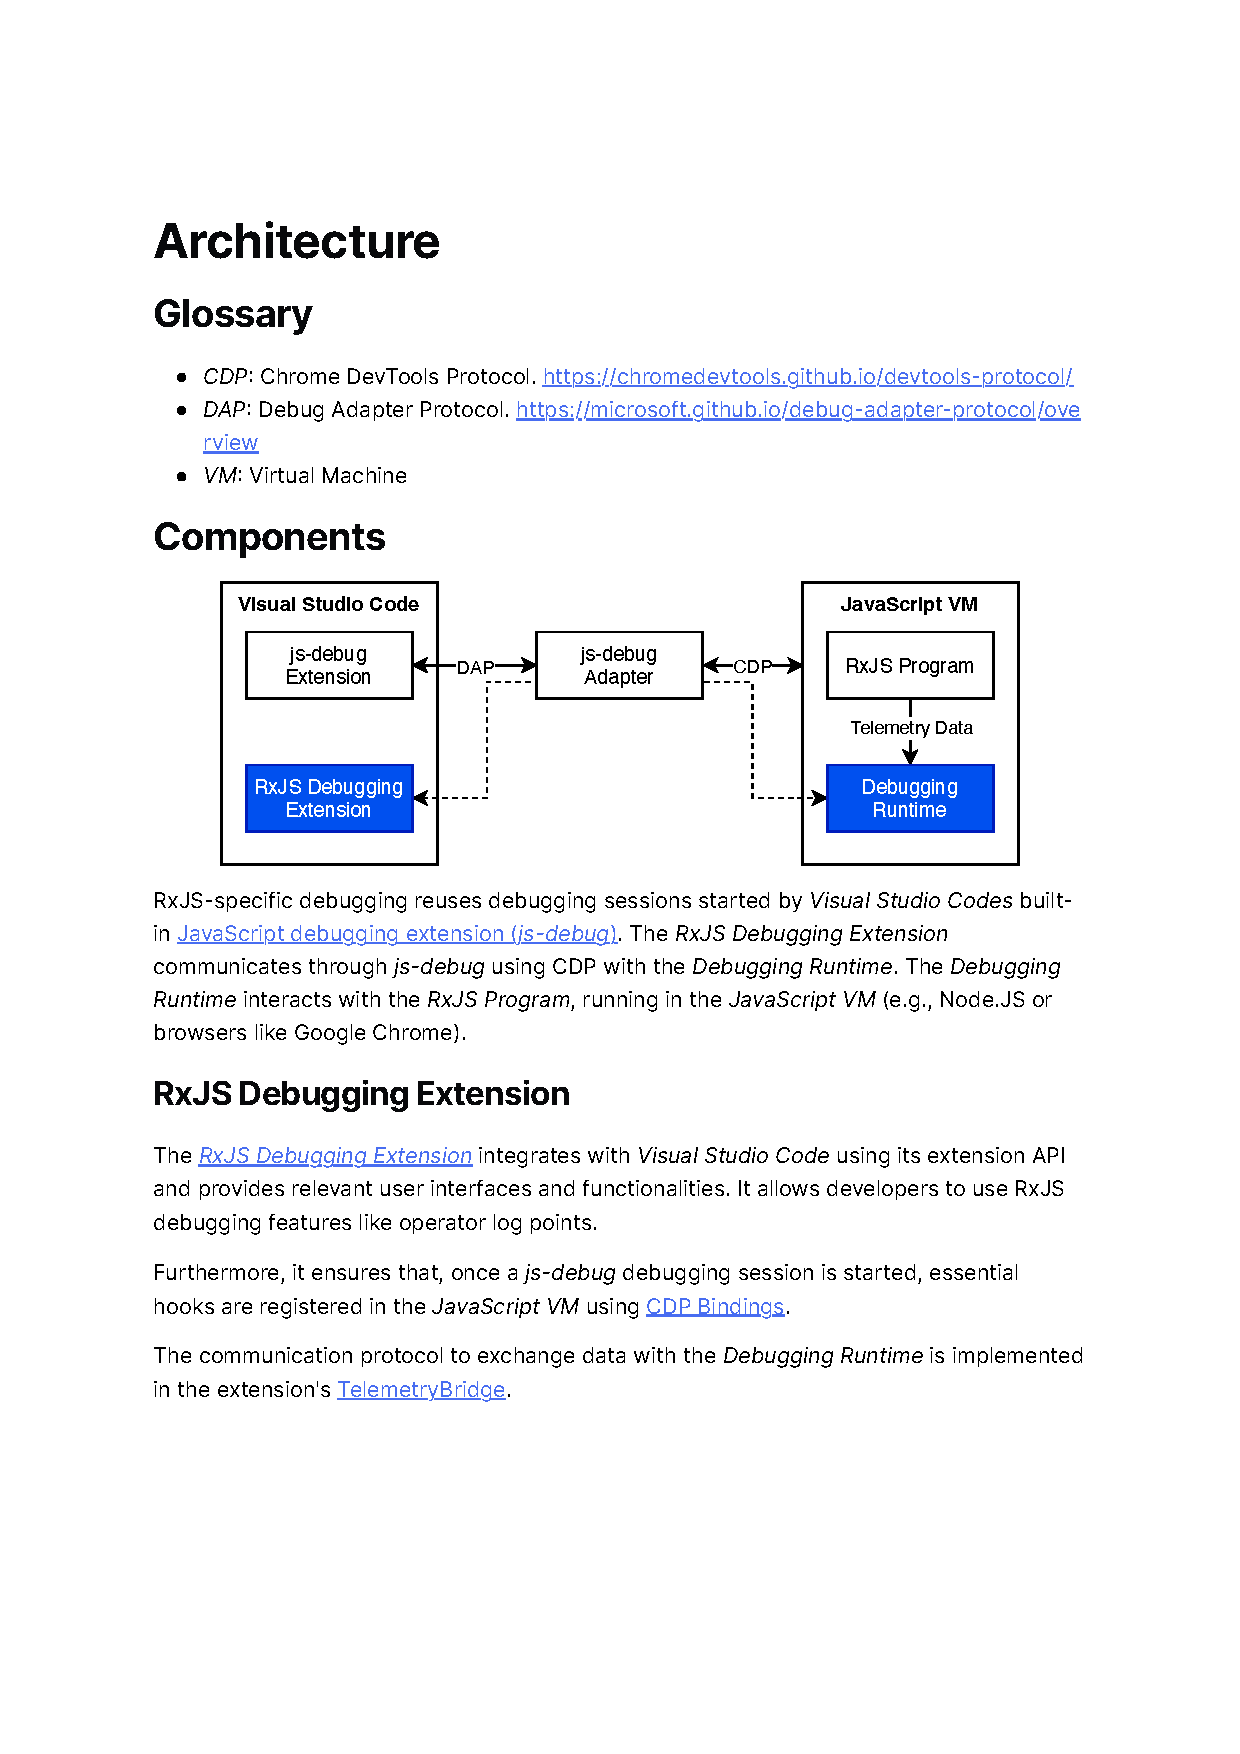
\includepdf[pages=-, landscape=true, nup=2, frame=true]{content/pdfs/architecturemd.pdf}


\subsection{CHANGELOG.md}
\label{sec:changelog}
The following document is a snapshot of the CHANGELOG.md file from the Git repository of RxJS Debugging for vscode:

\begin{itemize}
  \item \url{https://github.com/swissmanu/rxjs-debugging-for-vscode/blob/1cdb1579b872243a10747c94d9c623759dfa83f0/CHANGELOG.md}
\end{itemize}

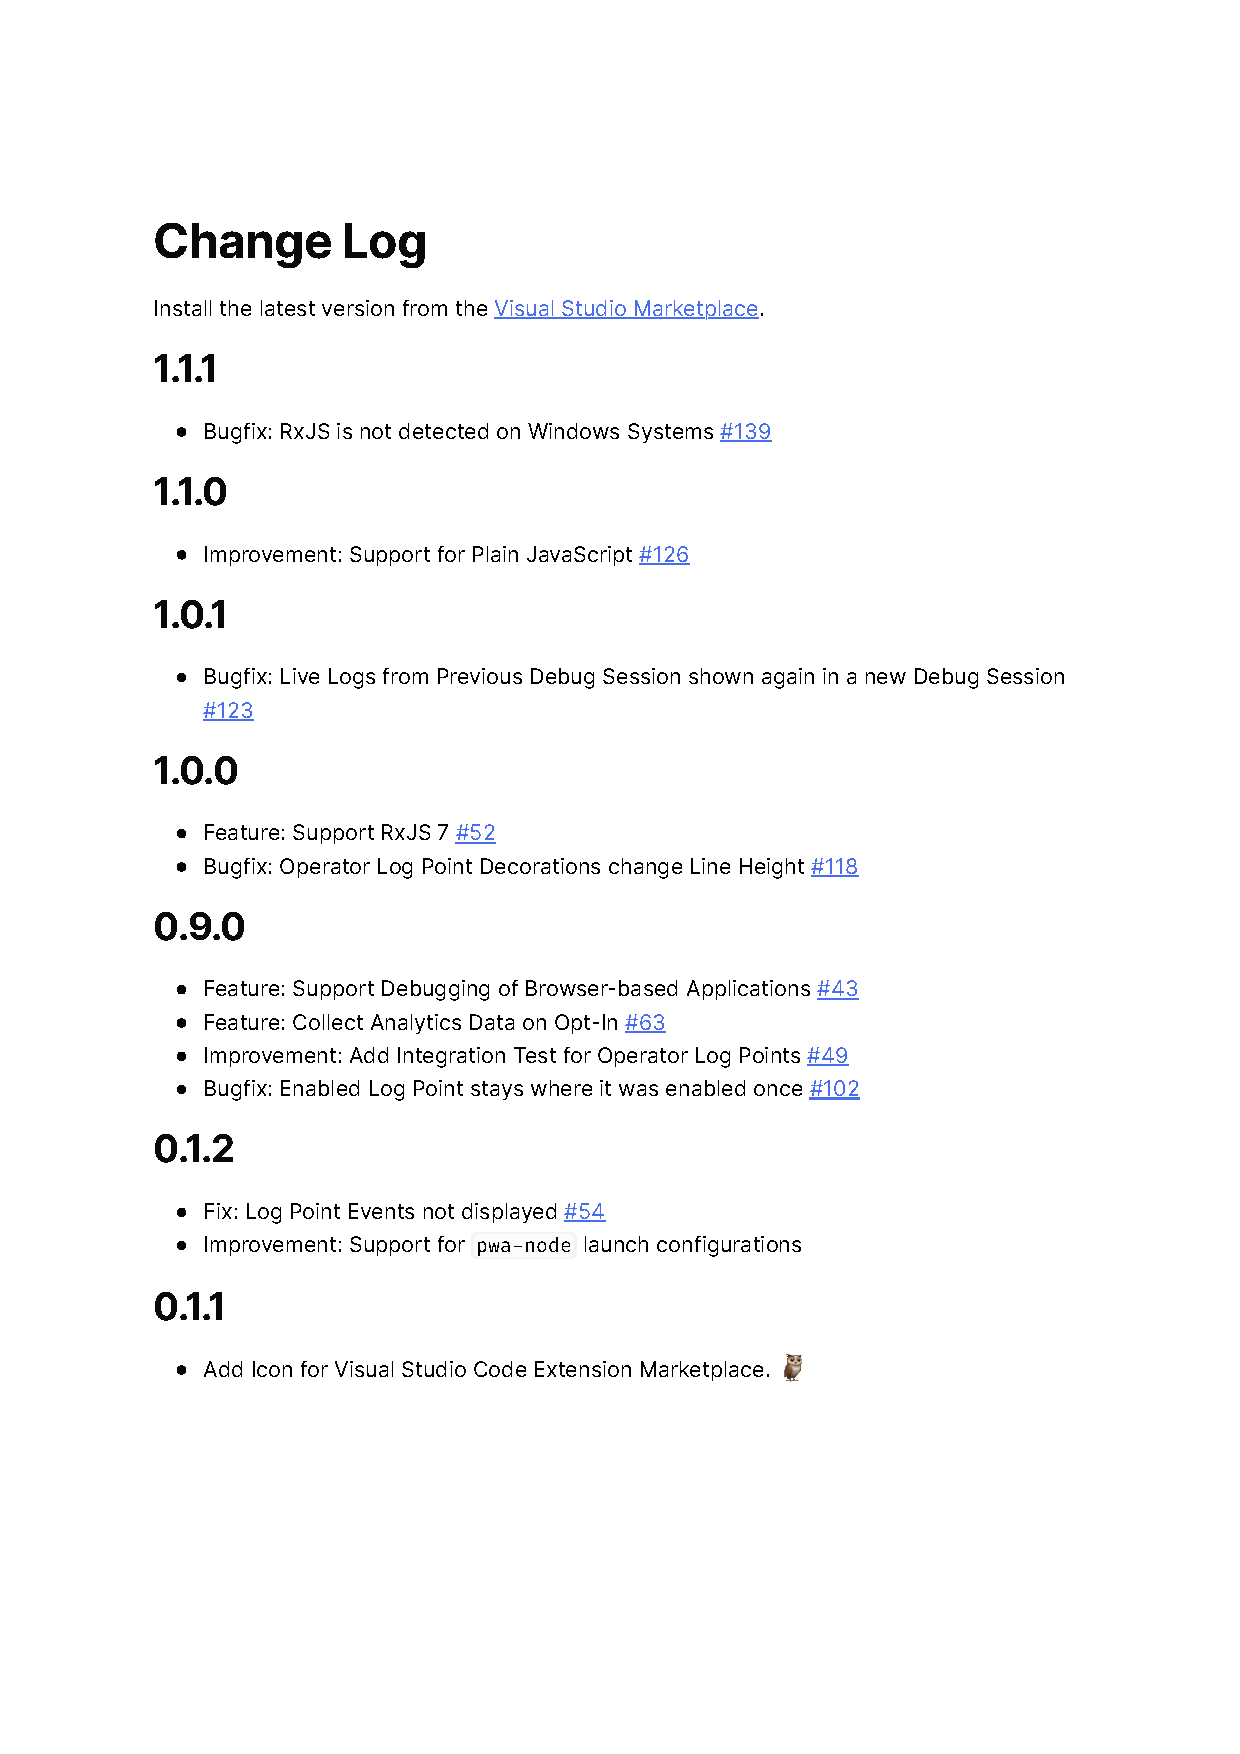
\includepdf[pages=-, landscape=true, nup=2, frame=true]{content/pdfs/changelogmd.pdf}



\subsection{CONTRIBUTING.md}
\label{sec:contributing}
The following document is a snapshot of the CONTRIBUTING.md file from the Git repository of RxJS Debugging for vscode:

\begin{itemize}
  \item \url{https://github.com/swissmanu/rxjs-debugging-for-vscode/blob/2da72e21a733c99522633d8477892f3b5b48113c/CONTRIBUTING.md}
\end{itemize}

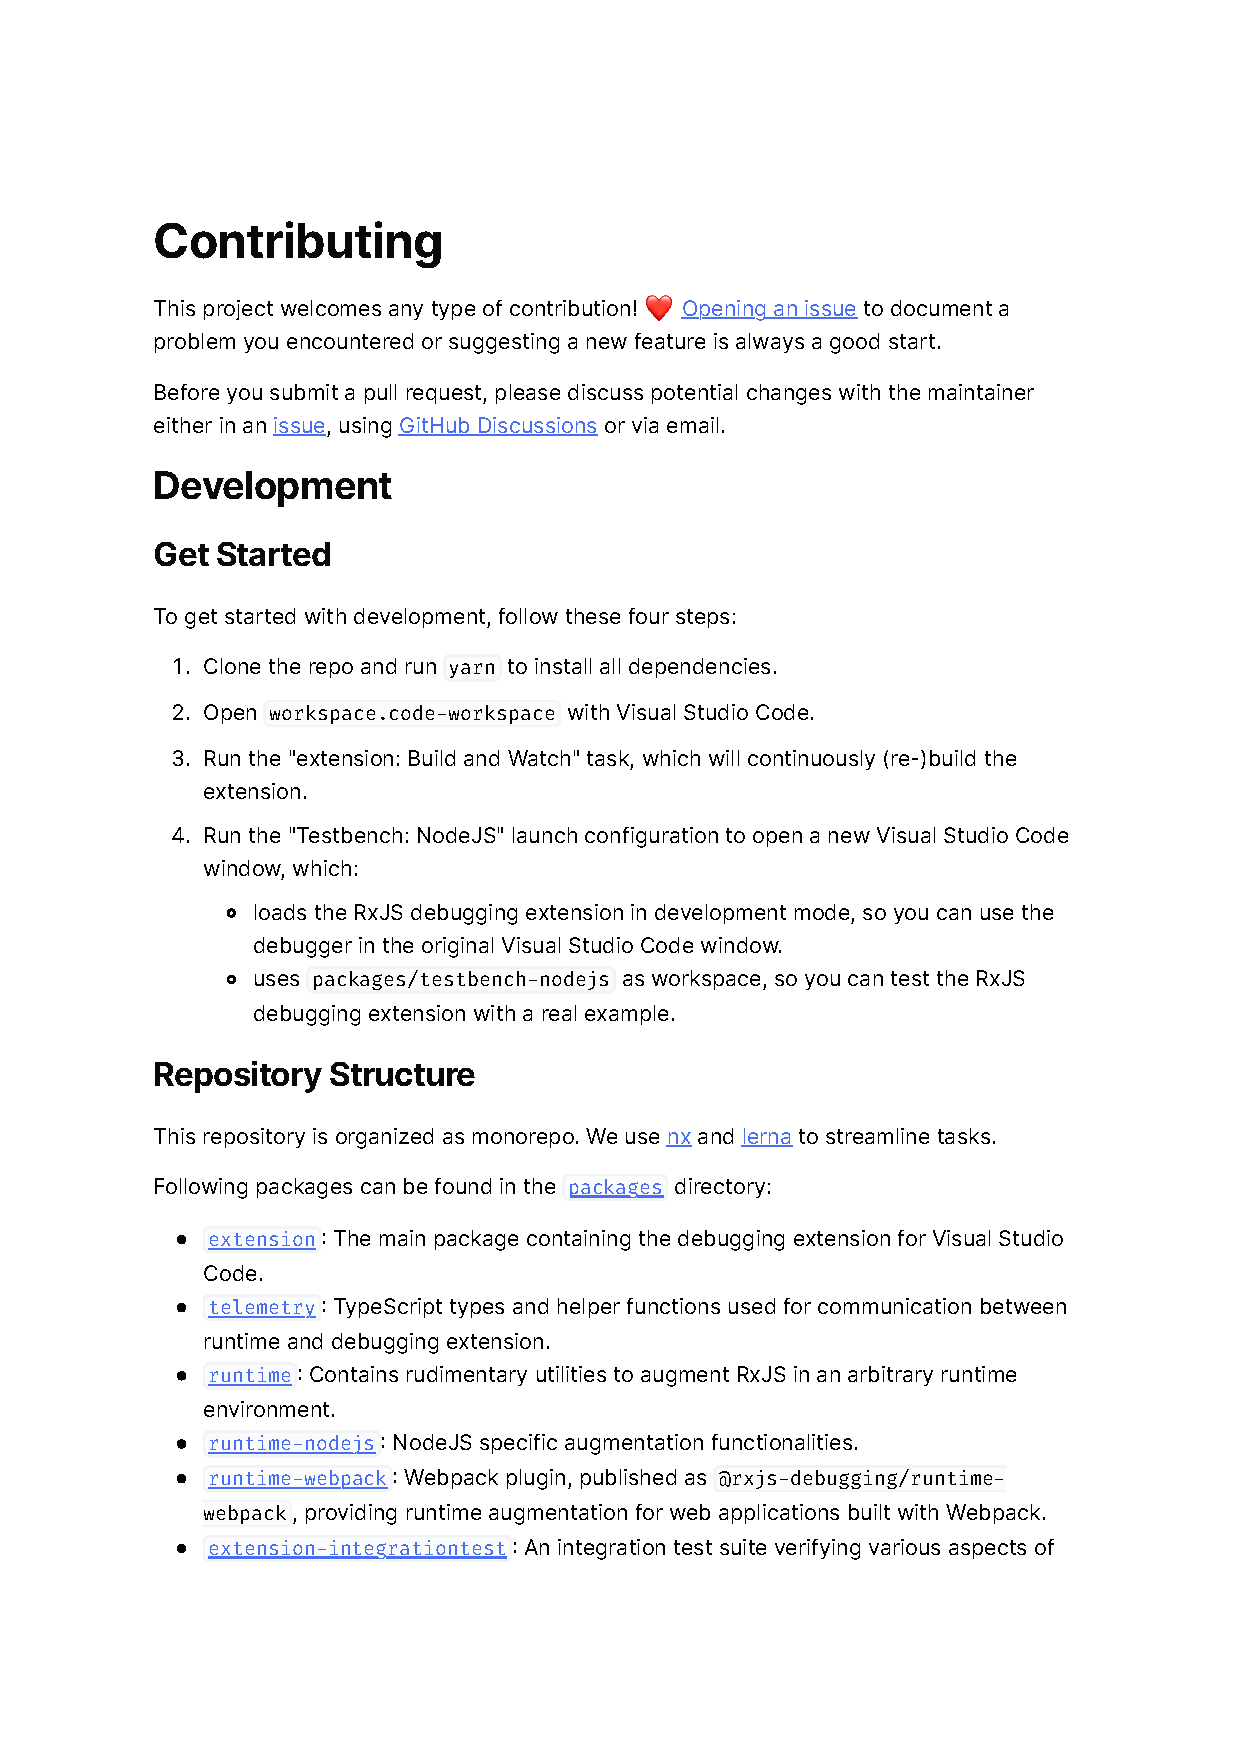
\includepdf[pages=-, landscape=true, nup=2, frame=true]{content/pdfs/contributingmd.pdf}



\subsection{Analytics Dashboard}
\label{sec:analytics-dashboard}
The following screenshot was taken at the 30th of December 2021, 19:00 CET.

As described in Appendix \ref{sec:analytics}, analytics data is not publicly accessible at this time.

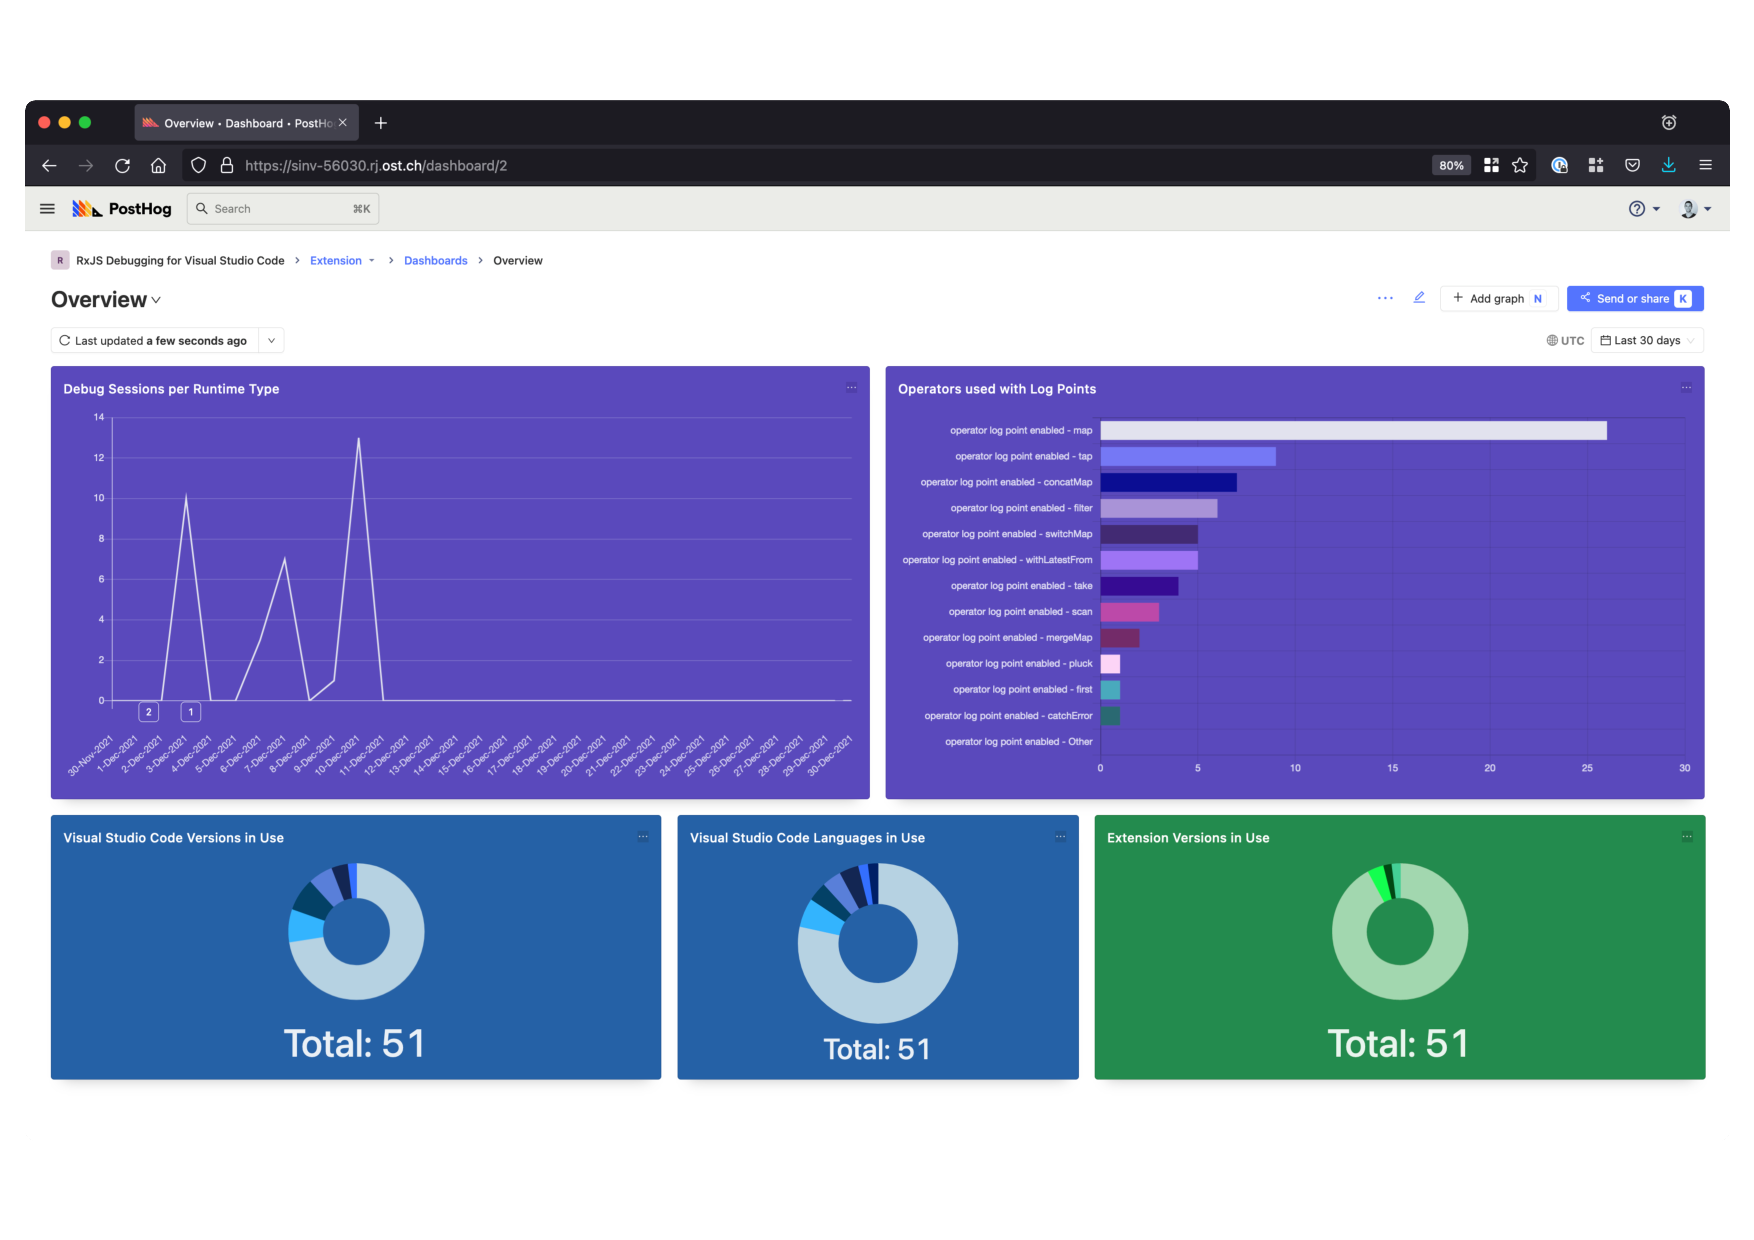
\includepdf[landscape=true, pages=-]{content/pdfs/posthog.pdf}



\section{vscode-js-debug Pull Request: Reuse CDP Connection}
\label{sec:cdp-pull-request}
The following document was created at the 31th of December, 10:00 CET and is publicly accesible:

\begin{itemize}
  \item \url{https://github.com/microsoft/vscode-js-debug/pull/964}
\end{itemize}

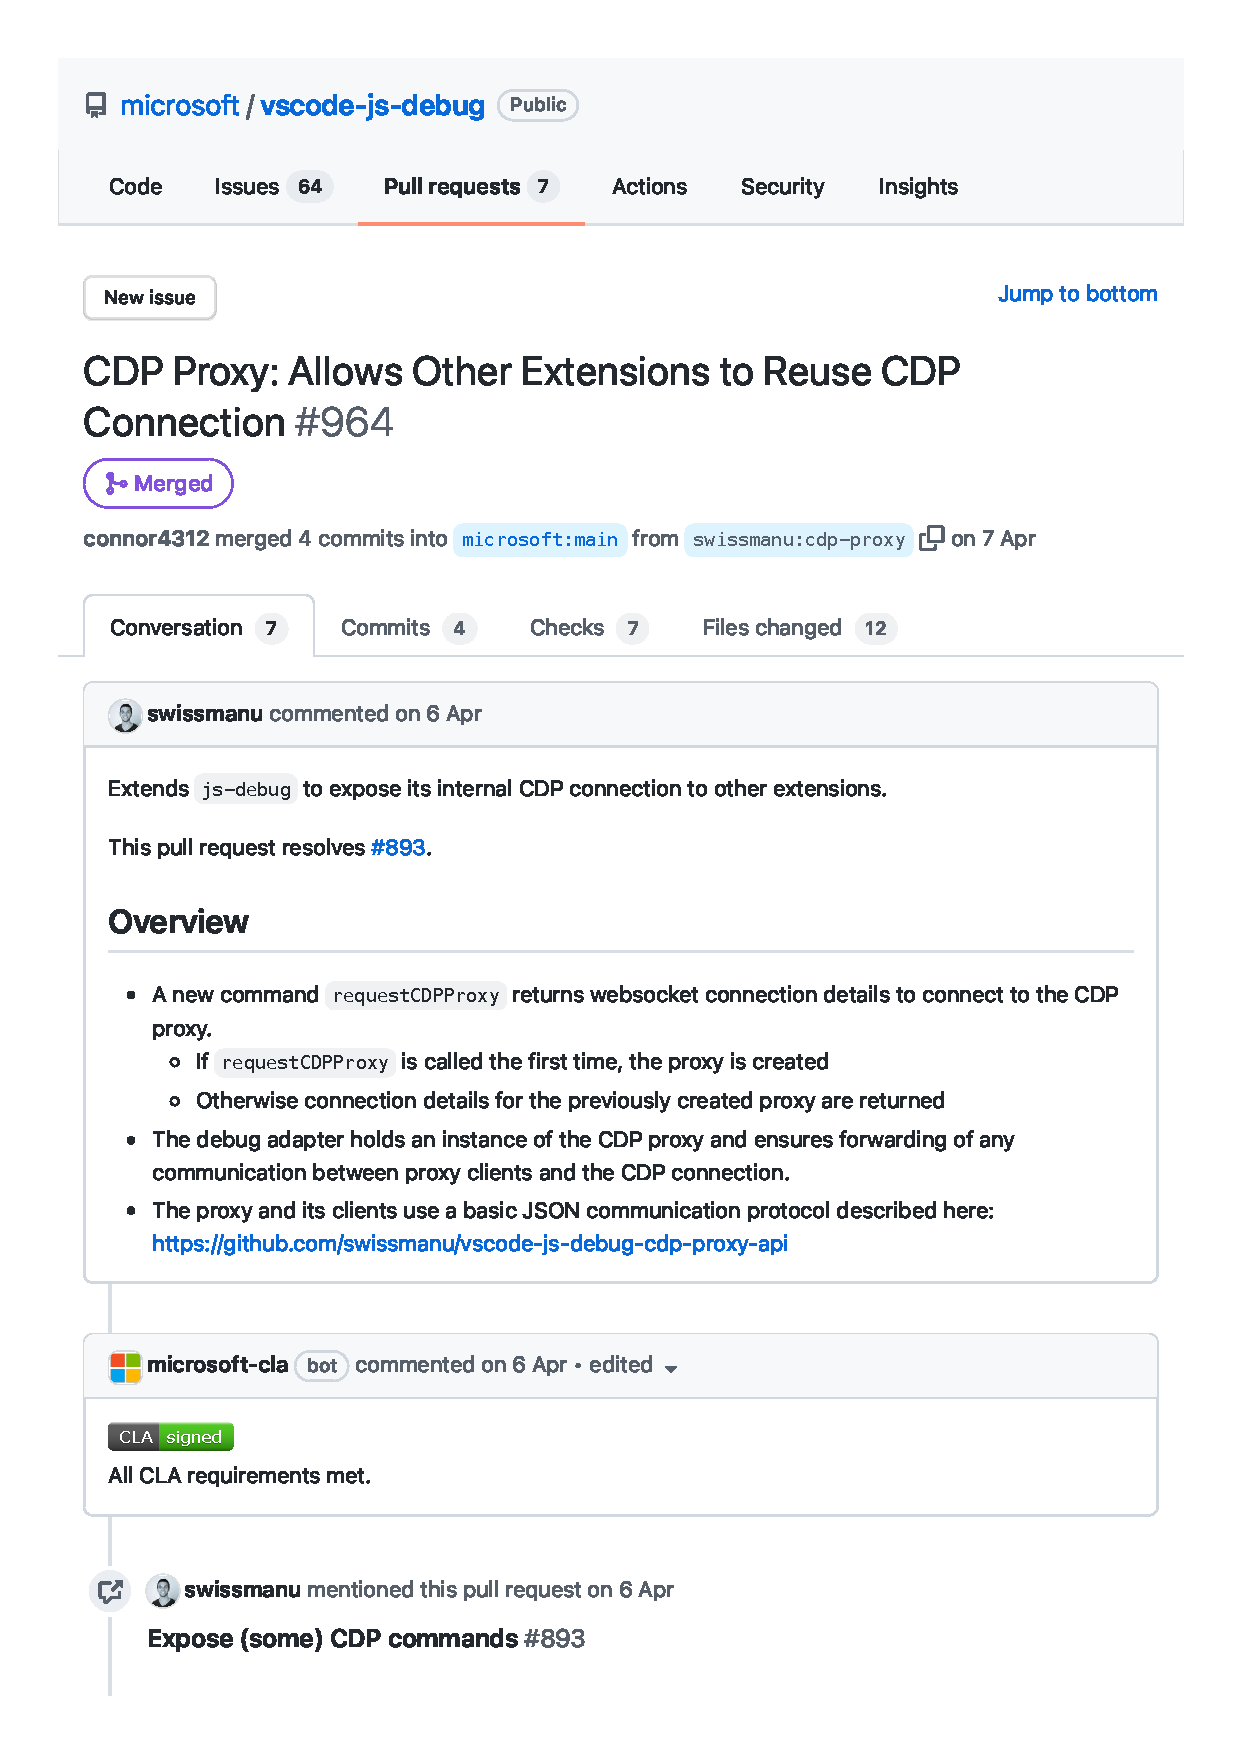
\includepdf[pages=-, landscape=true, nup=2, frame=true]{content/pdfs/cdp-pull-request.pdf}



\section{Open Science}
\label{sec:open-science}

\subsection{This Thesis}
\begin{itemize}
  \item \url{https://github.com/swissmanu/mse-thesis} \\ (publicly accessible by May 2022)
\end{itemize}

\subsection{Research Papers}
\begin{itemize}
  \item Debugging of RxJS-based Applications \\ \url{https://github.com/swissmanu/mse-paper-debugging-of-rxjs-based-applications}
  \item Debugging Support for Reactive Programming: Feasibility of a Ready-to-hand Debugger for RxJS \\ \url{https://github.com/swissmanu/mse-paper-rxjs-debugger} \\ (publicly accessible by May 2022)
\end{itemize}

\subsection{Studies}
\begin{itemize}
  \item Observational study \\ \url{https://github.com/swissmanu/mse-pa1-experiment}
  \item Usability test \\ \url{https://github.com/swissmanu/mse-pa2-usability-test}
\end{itemize}
